\documentclass[
12pt, % Main document font size
a4paper, % Paper type, use 'letterpaper' for US Letter paper
oneside, % One page layout (no page indentation)
%twoside, % Two page layout (page indentation for binding and different headers)
headinclude,footinclude, % Extra spacing for the header and footer
BCOR5mm, % Binding correction
]{scrartcl}

%%%%%%%%%%%%%%%%%%%%%%%%%%%%%%%%%%%%%%%%%
% Arsclassica Article
% Structure Specification File
%
% This file has been downloaded from:
% http://www.LaTeXTemplates.com
%
% Original author:
% Lorenzo Pantieri (http://www.lorenzopantieri.net) with extensive modifications by:
% Vel (vel@latextemplates.com)
%
% License:
% CC BY-NC-SA 3.0 (http://creativecommons.org/licenses/by-nc-sa/3.0/)
%
%%%%%%%%%%%%%%%%%%%%%%%%%%%%%%%%%%%%%%%%%

%----------------------------------------------------------------------------------------
%	REQUIRED PACKAGES
%----------------------------------------------------------------------------------------

\usepackage[
nochapters, % Turn off chapters since this is an article        
beramono, % Use the Bera Mono font for monospaced text (\texttt)
eulermath,% Use the Euler font for mathematics
pdfspacing, % Makes use of pdftex’ letter spacing capabilities via the microtype package
dottedtoc % Dotted lines leading to the page numbers in the table of contents
]{classicthesis} % The layout is based on the Classic Thesis style

\usepackage{arsclassica} % Modifies the Classic Thesis package

\usepackage[T1]{fontenc} % Use 8-bit encoding that has 256 glyphs

\usepackage[utf8]{inputenc} % Required for including letters with accents

\usepackage{graphicx} % Required for including images
\graphicspath{{Figures/}} % Set the default folder for images

\usepackage{enumitem} % Required for manipulating the whitespace between and within lists

\usepackage{lipsum} % Used for inserting dummy 'Lorem ipsum' text into the template

\usepackage{subfig} % Required for creating figures with multiple parts (subfigures)

\usepackage{amsmath,amssymb,amsthm} % For including math equations, theorems, symbols, etc

\usepackage{varioref} % More descriptive referencing

%----------------------------------------------------------------------------------------
%	THEOREM STYLES
%---------------------------------------------------------------------------------------

\theoremstyle{definition} % Define theorem styles here based on the definition style (used for definitions and examples)
\newtheorem{definition}{Definition}

\theoremstyle{plain} % Define theorem styles here based on the plain style (used for theorems, lemmas, propositions)
\newtheorem{theorem}{Theorem}

\theoremstyle{remark} % Define theorem styles here based on the remark style (used for remarks and notes)

%----------------------------------------------------------------------------------------
%	HYPERLINKS
%---------------------------------------------------------------------------------------

\hypersetup{
%draft, % Uncomment to remove all links (useful for printing in black and white)
colorlinks=true, breaklinks=true, bookmarks=true,bookmarksnumbered,
urlcolor=webbrown, linkcolor=RoyalBlue, citecolor=webgreen, % Link colors
pdftitle={}, % PDF title
pdfauthor={\textcopyright}, % PDF Author
pdfsubject={}, % PDF Subject
pdfkeywords={}, % PDF Keywords
pdfcreator={pdfLaTeX}, % PDF Creator
pdfproducer={LaTeX with hyperref and ClassicThesis} % PDF producer
} % Include the structure.tex file which specified the document structure and layout

\hyphenation{Fortran hy-phen-ation} % Specify custom hyphenation points in words with dashes where you would like hyphenation to occur, or alternatively, don't put any dashes in a word to stop hyphenation altogether

\usepackage{listings}
\usepackage{color}

\definecolor{dkgreen}{rgb}{0,0.6,0}
\definecolor{gray}{rgb}{0.5,0.5,0.5}
\definecolor{mauve}{rgb}{0.58,0,0.82}

\lstset{frame=tb,
	language=Java,
	aboveskip=3mm,
	belowskip=3mm,
	showstringspaces=false,
	columns=flexible,
	basicstyle={\small\ttfamily},
	numbers=none,
	numberstyle=\tiny\color{gray},
	keywordstyle=\color{blue},
	commentstyle=\color{dkgreen},
	stringstyle=\color{mauve},
	breaklines=true,
	breakatwhitespace=true,
	tabsize=3
}

%----------------------------------------------------------------------------------------
%	TITLE AND AUTHOR(S)
%----------------------------------------------------------------------------------------

\title{\normalfont\spacedallcaps{Final Project of Automata Theory}} % The article title

%\subtitle{Subtitle} % Uncomment to display a subtitle

\author{\spacedlowsmallcaps{Amin Mohammad Soleimani Abyaneh 94100805\textsuperscript{1}}} % The article author(s) - author affiliations need to be specified in the AUTHOR AFFILIATIONS block

\date{} % An optional date to appear under the author(s)

%----------------------------------------------------------------------------------------

\begin{document}

%----------------------------------------------------------------------------------------
%	HEADERS
%----------------------------------------------------------------------------------------

\renewcommand{\sectionmark}[1]{\markright{\spacedlowsmallcaps{#1}}} % The header for all pages (oneside) or for even pages (twoside)
%\renewcommand{\subsectionmark}[1]{\markright{\thesubsection~#1}} % Uncomment when using the twoside option - this modifies the header on odd pages
\lehead{\mbox{\llap{\small\thepage\kern1em\color{halfgray} \vline}\color{halfgray}\hspace{0.5em}\rightmark\hfil}} % The header style

\pagestyle{scrheadings} % Enable the headers specified in this block

%----------------------------------------------------------------------------------------
%	TABLE OF CONTENTS & LISTS OF FIGURES AND TABLES
%----------------------------------------------------------------------------------------

\maketitle % Print the title/author/date block

\setcounter{tocdepth}{2} % Set the depth of the table of contents to show sections and subsections only

\tableofcontents % Print the table of contents

\listoffigures % Print the list of figures

\let\thefootnote\relax\footnotetext{* \textit{Department of Computer Science, Sharif University of Technology}}

%----------------------------------------------------------------------------------------

\newpage 

\section{Introduction}
Automata theory is a theoretical field in CS, which mainly discusses the logic of computation with respect to basic and abstract machines, called automata.This study enables the scientists to understand the computers are able to comprehend the functions and solve difficult problems. In this context, we are mainly engaged in dealing with Finite State Machines, e.g. DFA and NFA, and Push Down Automata. As we already know, the Deterministic Finite Automata (DFA) and Non-deterministic Finite Automata(NFA) are employed to recognize a Regular Language while PDA is used to process a Context Free Language.

In this project, we are supposed to deliver three main algorithms which we have studied during the course. The main code consists of an I/O interface in command line which implements the desired input and output handling. In each of the next sections we present one of the following problems of the project. The three main functions that we have to implement are as the following.

\begin{itemize}
	\item Convert a Regular Expression to NFA and vice versa.
	\item Conversion of NFA to DFA and ultimately to minimum DFA.
	\item Conversion of a Context Free Grammar to PDA.
\end{itemize}

The source project is also available in \url{https://github.com/aminabyaneh/Automata_Theory}. The repository also contains some simple and complex test cases, as well as the development history and corresponding algorithms.

\paragraph{Warning} The source code is implemented entirely in JAVA 11, so using lower versions of Java to run the code may cause unanticipated errors and warnings. The code is also explained in the sub-section of each respective task and the required objects and functions are mentioned under the sub-section of implementation, however, it also contains a comprehensive Javadoc which is attached to this report.

\newpage
\section{General Structure of the Code}
The code consists of several parts ranging from input handling to various automata algorithms. To chase the structure of the code, one should start with the function $automata()$, called in the main. This function is a state machine responding to various types of input data. The class $IO$ is responsible for handling the input and output methods, which first reads the first line, and then calls a corresponding functions based on the type of the input: Regex, NFA, or CFG. 

The code then creates a container which stores the values of input into one of the following classes: $CFGEntry$, $NFAEntry$, and $RegExEntry$ which are all children of the super class $Entry$. These containers store the data and provide a complete set of functions to manipulate the entry data. And, are passed to the corresponding objects to generate the data needed for the algorithms.

Afterward, there are again three main objects: $DFA$, $NFA$, and $CFG$, where $DFA$ and $NFA$ are children of a super abstract class called $FSM$. These classes all have a field of the object $StateTransitionMatrix$ which is the state transition matrix of the object. State transition matrix is a class that uses inheritance to build a 3-dimensional ArrayList. Each column is implemented as a 2-dimensional ArrayList and contains number of cells which are all 1-dimensional ArrayLists. In addition to the matrix, each of the mentioned classes comprise of a set of functions to implement algorithms like building NFA from Regex and creating the minimum DFA. For determining the structure, it is also useful to look at the following code snippet. 
\begin{lstlisting}
/** The main automata function. */
private static void automata() {
IO ioHandler = new IO();
switch (ioHandler.getDataType()) {

case RegEx:
RegEx regEx = new RegEx((RegExEntry)ioHandler.getData());
regEx.taskHandler();
break;
case NFA:
NFA nfa = new NFA((NFAEntry)ioHandler.getData());
nfa.taskHandler();
break;
case CFG: 
CFG cfg = new CFG((CFGEntry)ioHandler.getData());
cfg.taskHandler();
default:
break;
	}
}
\end{lstlisting}


\newpage
\section{Regular Expression to NFA and Vice Versa}
In this section, we investigate the procedure of converting RE to NFA and vice versa. We first explain the forward direction of the problem and later explain the postulated reverse direction.
\subsection{Regular Expression to NFA}
To convert a regular expression to an NFA, we have to follow a recursive procedure based on Thompson construction rules. The recursion reduces the computation complexity and divides the problem into more understandable sub-problems which are then solved by constructing a trivial Automata. In the next sections we first discuss the algorithm behind the scene, then explain the implementation and finally the input output structures and the results.
\subsubsection{Algorithm}
To convert a Regex to NFA, we go through several stages. The goal is to parse the Regex correctly and break the expression recursively to reach trivial NFA, and then merge the NFAs into the final NFA. To build up the final NFA, we break down the Regex to one of the following situations in Figure~\vref{fig:Thompson}. As it appears from the figure, each cas 1 to 4 corresponds to an special case of operations which is listed here.

\begin{enumerate}
	\item The trivial NFA, where we only have a symbol like $a$ or $b$.
	\item The union NFA, whenever we have two NFAs like $N(s)$ and $N(t)$, we construct the NFA of $N(s) | N(t)$ like this.
	\item The concatenation NFA, whenever we have two NFAs like $N(s)$ and $N(t)$, we construct the NFA of $N(s).N(t)$ like the picture.
	\item The start NFA, whenever we have a NFA like $N(s)$, we construct the NFA of $N(s)^{*}$ like mentioned in the picture.
\end{enumerate}

\begin{figure}[tb]
	\centering 
	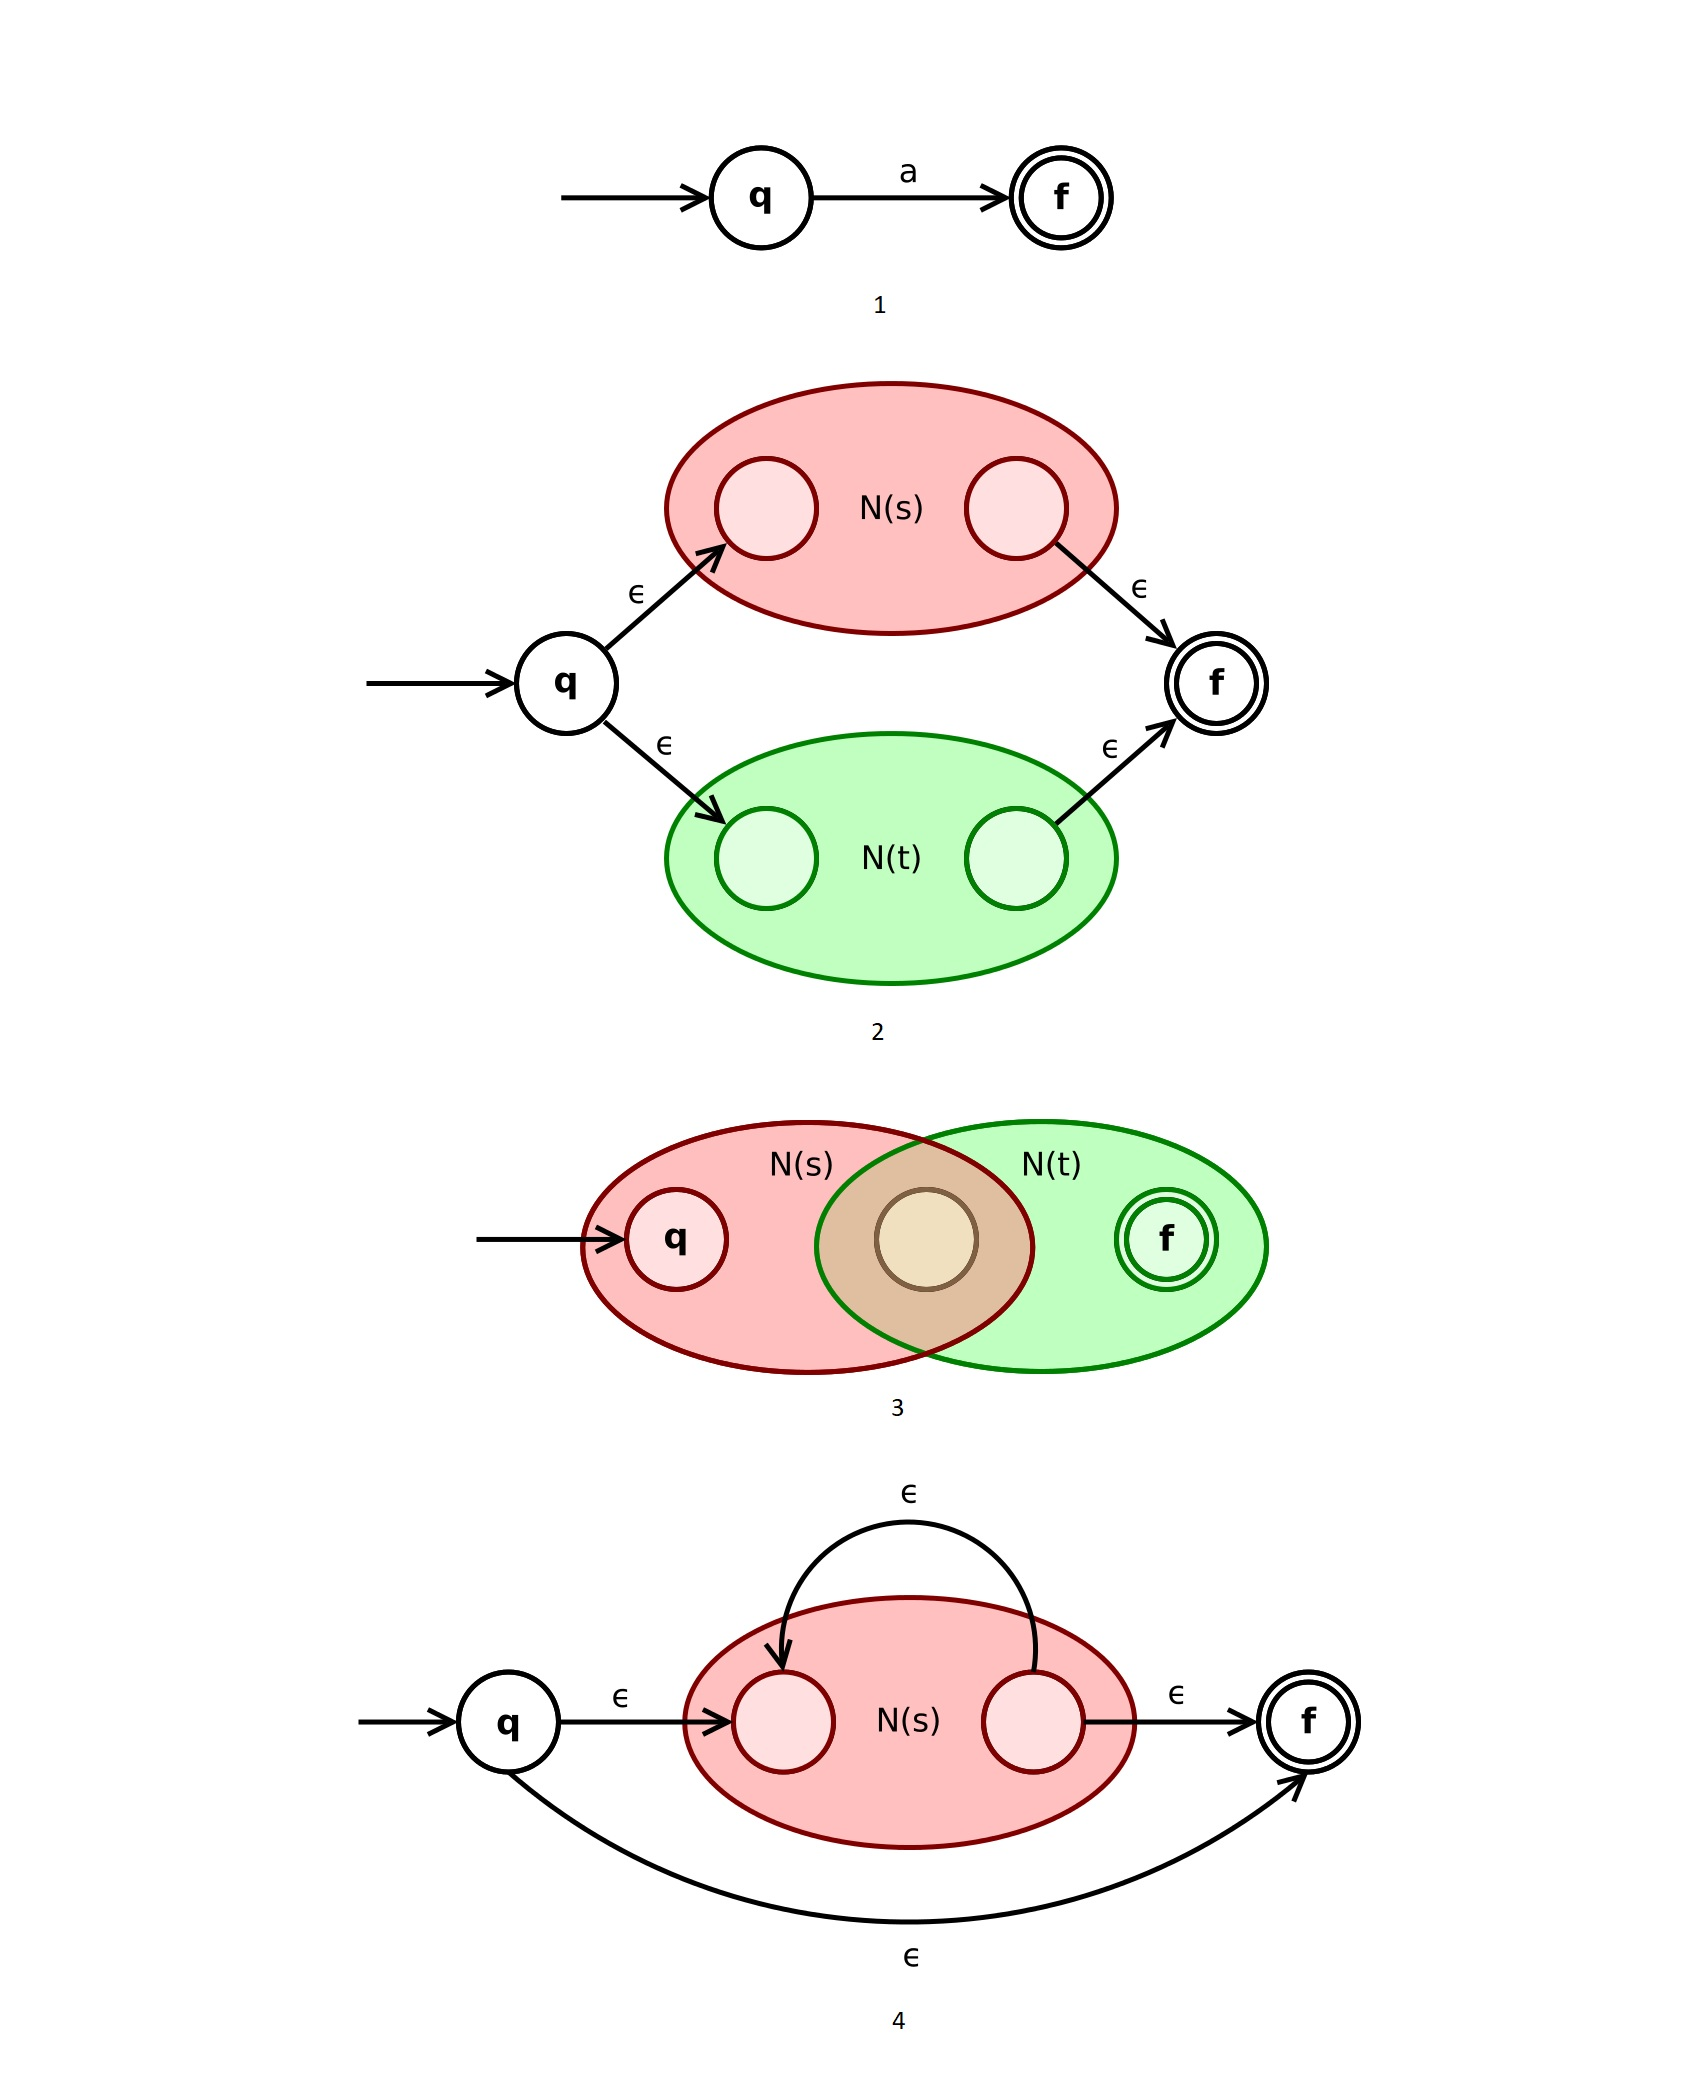
\includegraphics[width=0.8\columnwidth]{Thompson} 
	\caption[]{Thompson construction rules}
	\label{fig:Thompson} 
\end{figure}

\begin{figure}[tb]
	\centering 
	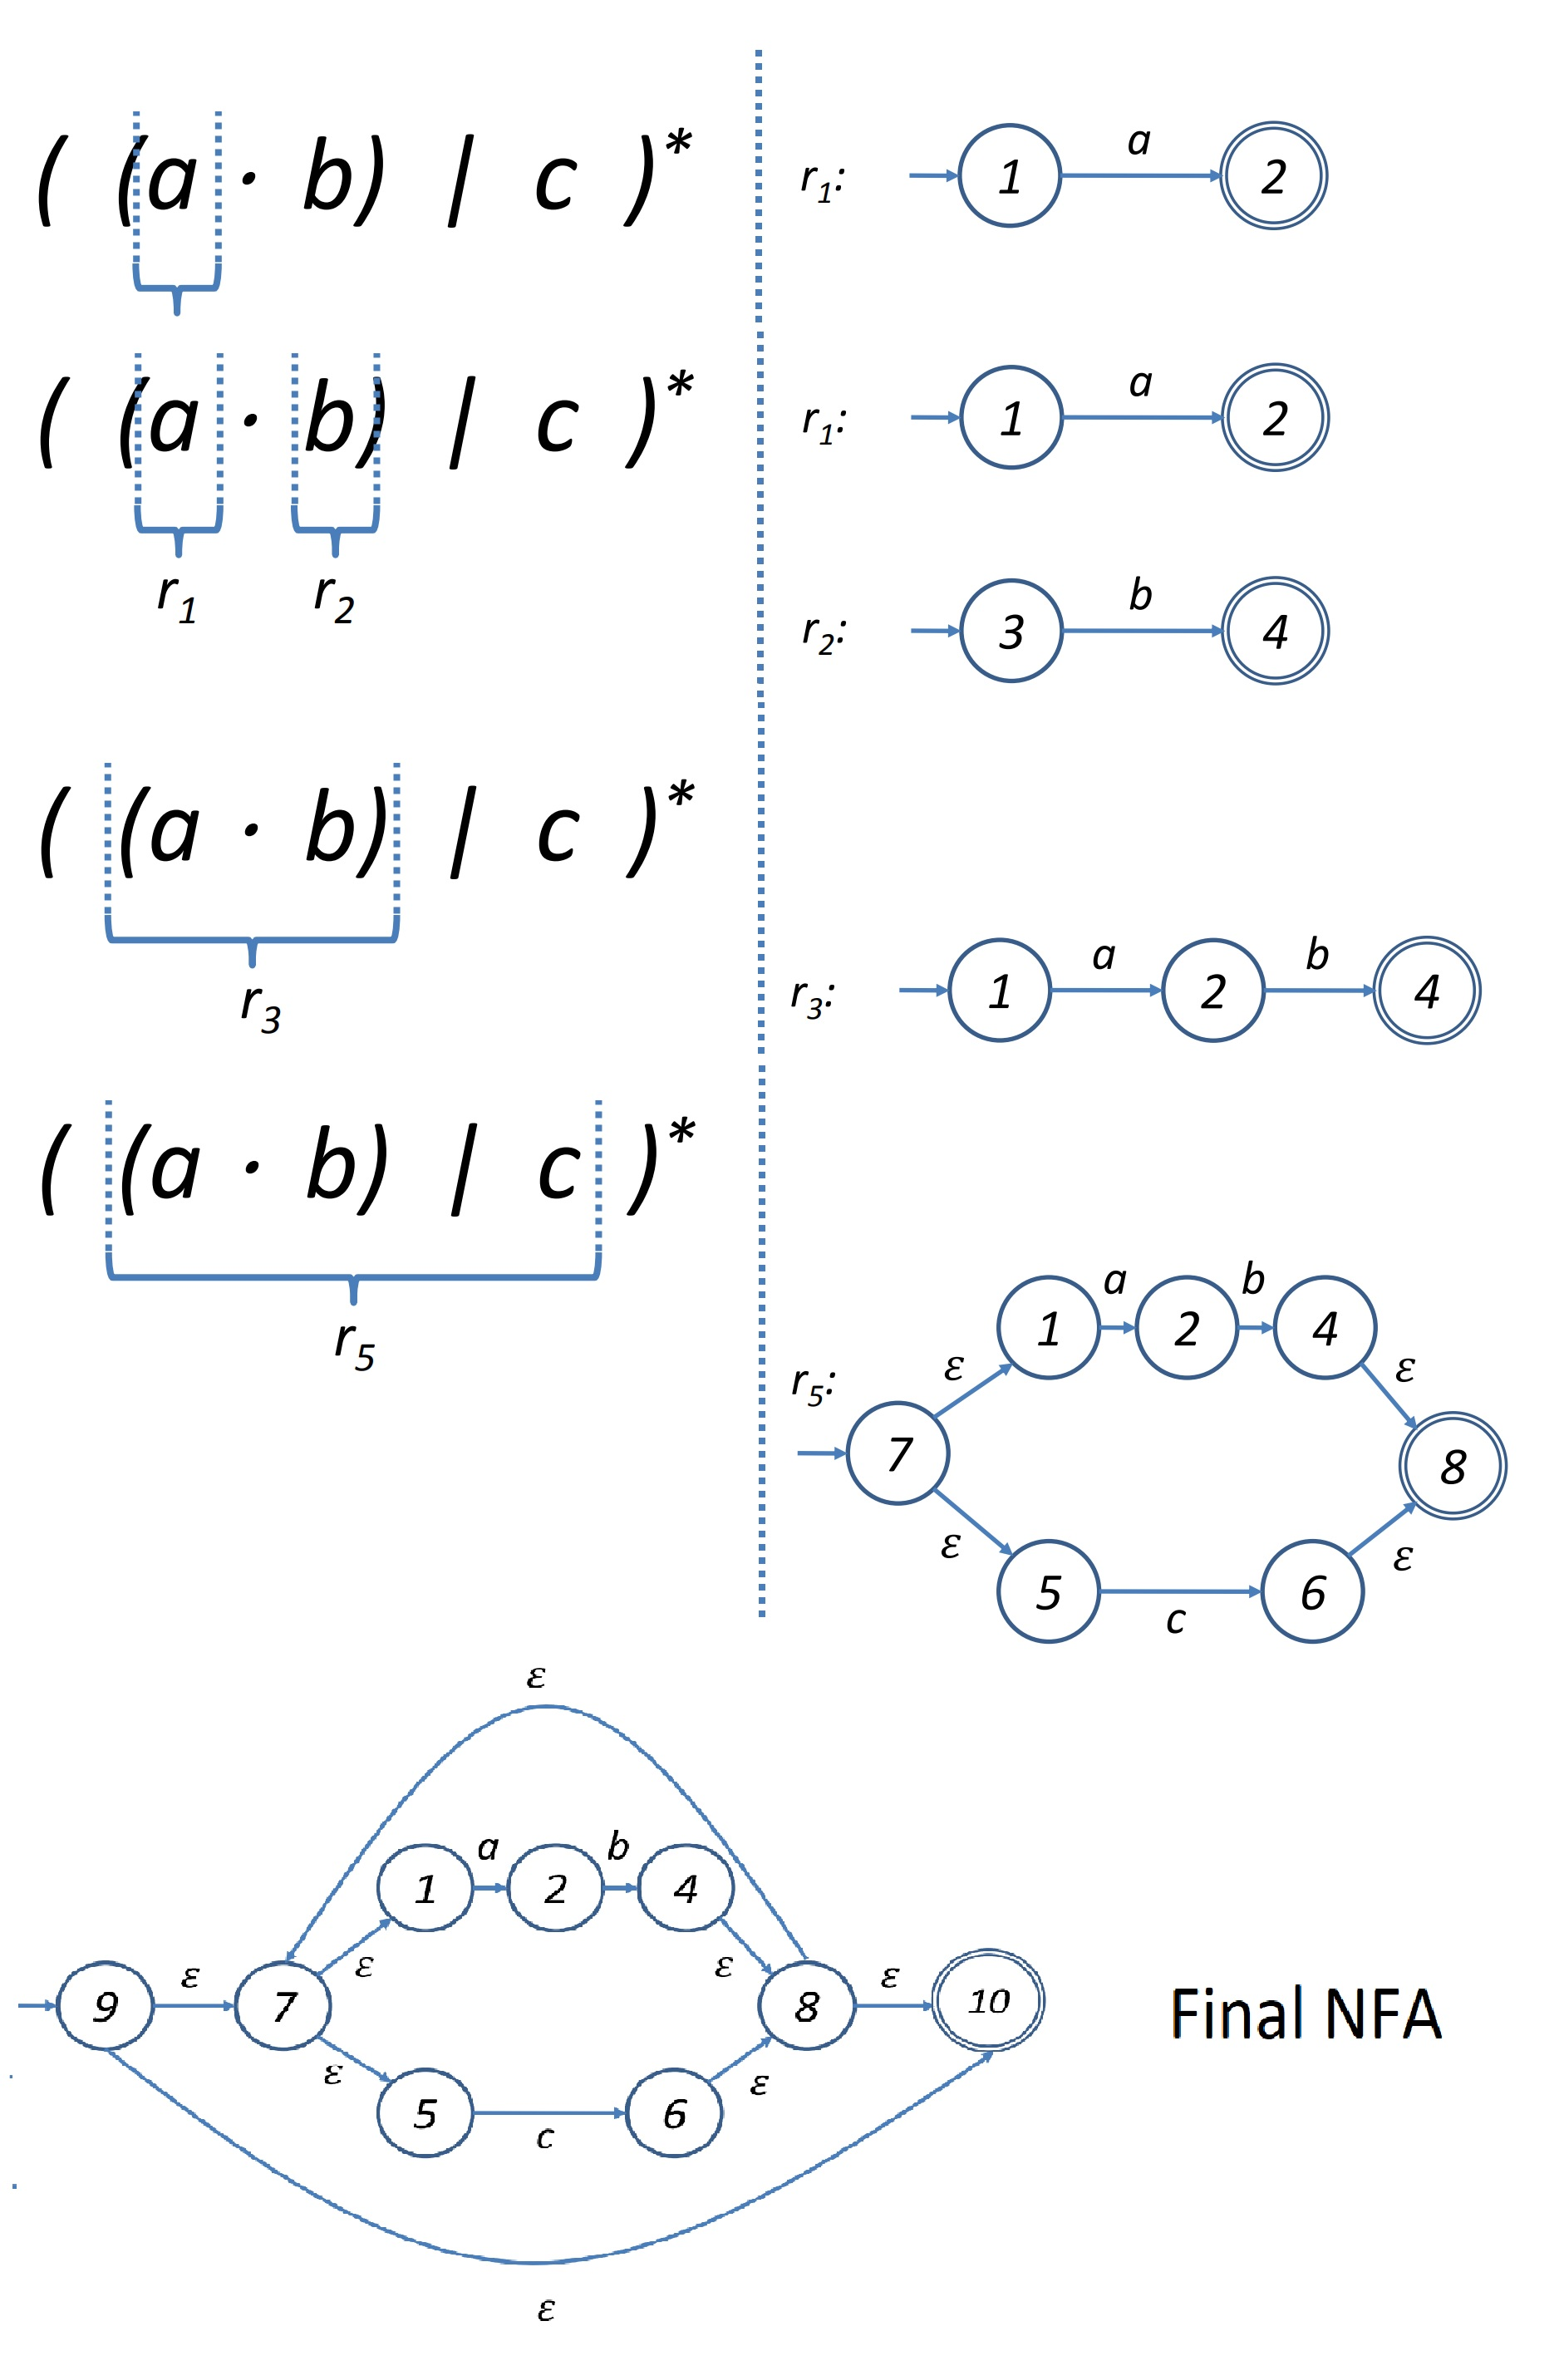
\includegraphics[width=0.8\columnwidth]{Thompson_procedure} 
	\caption[]{Thompson construction procedure}
	\label{fig:Thompson_procedure} 
\end{figure}

To further illustrate the algorithm, consider the Figure~\vref{fig:Thompson_procedure}. Here you can se that we first have to break down the regular expression down to the trivial Automata, i.e. case 1 in Figure~\vref{fig:Thompson}, and then step up merging Automatas based on case 2 to 4 in Figure~\vref{fig:Thompson}. 

\subsubsection{Implementation}
The implementation consists of several stages which are explained one by one in this section. The main function in this case generates a Regex object and Regex entry class to store and manipulate the input data. Then the following stages come along. The first step is to call the function $createNFA()$ in the $RegEx$ class. 

\paragraph{Reform the input Regex}
Here we add the symbol "." whenever there is a need for concatenation. By doing this we add "." to the set of operations that we already have, ${|, *}$. This is done by the function $addConcatenation()$. We also add parenthesis down to even a single symbol to make the processing more smooth using the $addParenthesis()$ function. The code snippet in the next page is a more clear example of what is really happening in the $creatNFA()$ function. Remember that after building the NFA we have to add the start and final state to the $requestedNFA$ object which we are going to return.

\newpage
\begin{lstlisting}
/**
* Creates the NFA. This function constructs and NFA recursively and
* returns the result.
*/
private NFA createNFA() {

	this.regex = this.addConcatenation();
	this.regex = this.addParenthesis();
	
	/** Build NFA from RegEx recursively. */
	NFA requestedNFA = this.buildNFA(this.regex);
	
	/** Set start and final state as they are first and last state. */
	ArrayList<Integer> finalStates = new ArrayList<Integer>();
	finalStates.add(requestedNFA.stmat.size() - 1);
	
	requestedNFA.setStartState(1);
	requestedNFA.setFinalStates(finalStates );
	
	return requestedNFA;
}
\end{lstlisting}

\paragraph{Building the NFA}
Now that we have reformed the Regex, we pass it to the function $buildNFA$. This function is a recursive function that creates the it is time to wrap it as a $Phrase$ object. The build function first checks the trivial case, which is when the Regex length is equal to 1, and then uses the function $extractPhrases(regex)$ to return the phrases inside a regex. Phrases are part of a regex with the lowest and same parenthesis priority. One may notice that when we are extracting the phrases, there based on the reformation which we performed previously, all the phrases with the same priority have the same operation between them, e.g., the operation between all of them is concatenation or union. Next, the function begins to check whether the phrases have the Kleene star or not. If it is the case, the code performs the $starNFA(NFA nfa)$ function which then applies the star to the nfa and returns the starred nfa. Similarly, the $concatNFA(nfaA, nfaB)$ function and the $unionNFA(nfaA, nfaB)$ function are used to build the concatenation and union results. This is explained in details in the next paragraph.

\paragraph{Micro Operations}
By convention, we call micro operations as the operations that are based on Thompson construction rules. To perform these kinds of operations, we need to apply the changes in the state transition matrix. To illustrate the method, let us consider the function $buildUnionNFA(stmA, stmB)$ in $StateTransitionMatrix$. This functions works similar to other functions building concatenation and star operation. First, there are two NFAs which we want to perform union operation on. We pass their state transition matrix to the function $buildUnionNFA(stmA, stmB)$. Then, inside the function, we first increment the state numbers if stmB and then merge it with stmA. Merging is done in a way that satisfies case 2 of the Figure~\vref{fig:Thompson}. At the end, two start and end states are added to the table and connect the two previous NFAs via epsilon, simulating the union function based on Thompson rules. The following code snippet may help the reader to understand the concept of micro operations on the state transition matrices.

\begin{lstlisting}
/** Building the state transition matrix for union NFA. */

/** Increment state numbers to add the new states. */
StateTransitionMatrix.incrementStateNumbers(nfaA);

/** Add two new states for the start and for the end. */
ArrayList<ArrayList<Integer>> startColumn =
new ArrayList<ArrayList<Integer>>();
ArrayList<ArrayList<Integer>> firstColumn =
nfaA.stmat.get(1);

/** Adding the start state to the beginning of state transition matrix. */
Integer index = -1;
for (ArrayList<Integer> c : firstColumn) {

	index++;
	changeCell = new ArrayList<Integer>();
	
	if (index == 0)
		changeCell.add(c.get(0) - 1);
	else if (index == firstColumn.size() - 1)
		changeCell.addAll(startStates);
	
	startColumn.add(changeCell);
}
\end{lstlisting}

\subsubsection{Results}
In this subsection, we present some of the major results of the implementation on some arbitrary regular expressions. The input output of the console are aligned with the regulations in the document provided with the project. Here we see results for three regular expression, from simple to rather complicated ones. The results are shown in Figure~\vref{fig:regextonfaresults}.

\begin{figure}[tb]
	\centering
	\subfloat[A city market.]{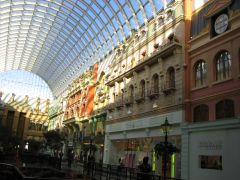
\includegraphics[width=.45\columnwidth]{Lorem}} \quad
	\subfloat[Forest landscape.]{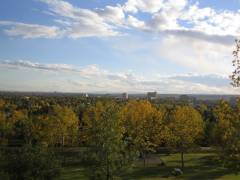
\includegraphics[width=.45\columnwidth]{Ipsum}\label{fig:ipsum}} \\
	\subfloat[Mountain landscape.]{
\includegraphics[width=.45\columnwidth]{Dolor}} \quad
	\subfloat[A tile decoration.]{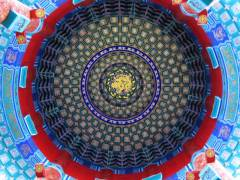
\includegraphics[width=.45\columnwidth]{Sit}}
	\caption[Results]{Results of the Regex to NFA converter}
	\label{fig:regextonfaresults}
\end{figure}

\subsection{NFA to Regular Expression}
\subsubsection{Algorithm}
\subsubsection{Implementation}
\subsubsection{Results}

\section{NFA to Minimum DFA}
This is the second required task of the project which comprises of two main sections: creating a DFA from a given NFA, conversion of DFA to minimum DFA. The methods related to this part of the project are implemented inside the $DFA$ object. In each section, we use a given algorithm to convert an FSM to another FSM with certain specifications. We investigate each of the major parts of the algorithm in the next two sections. A picture of the conversion sequence may be found in Figure~\vref{fig:nfatomindfa}.

\begin{figure}[tb]
	\centering 
	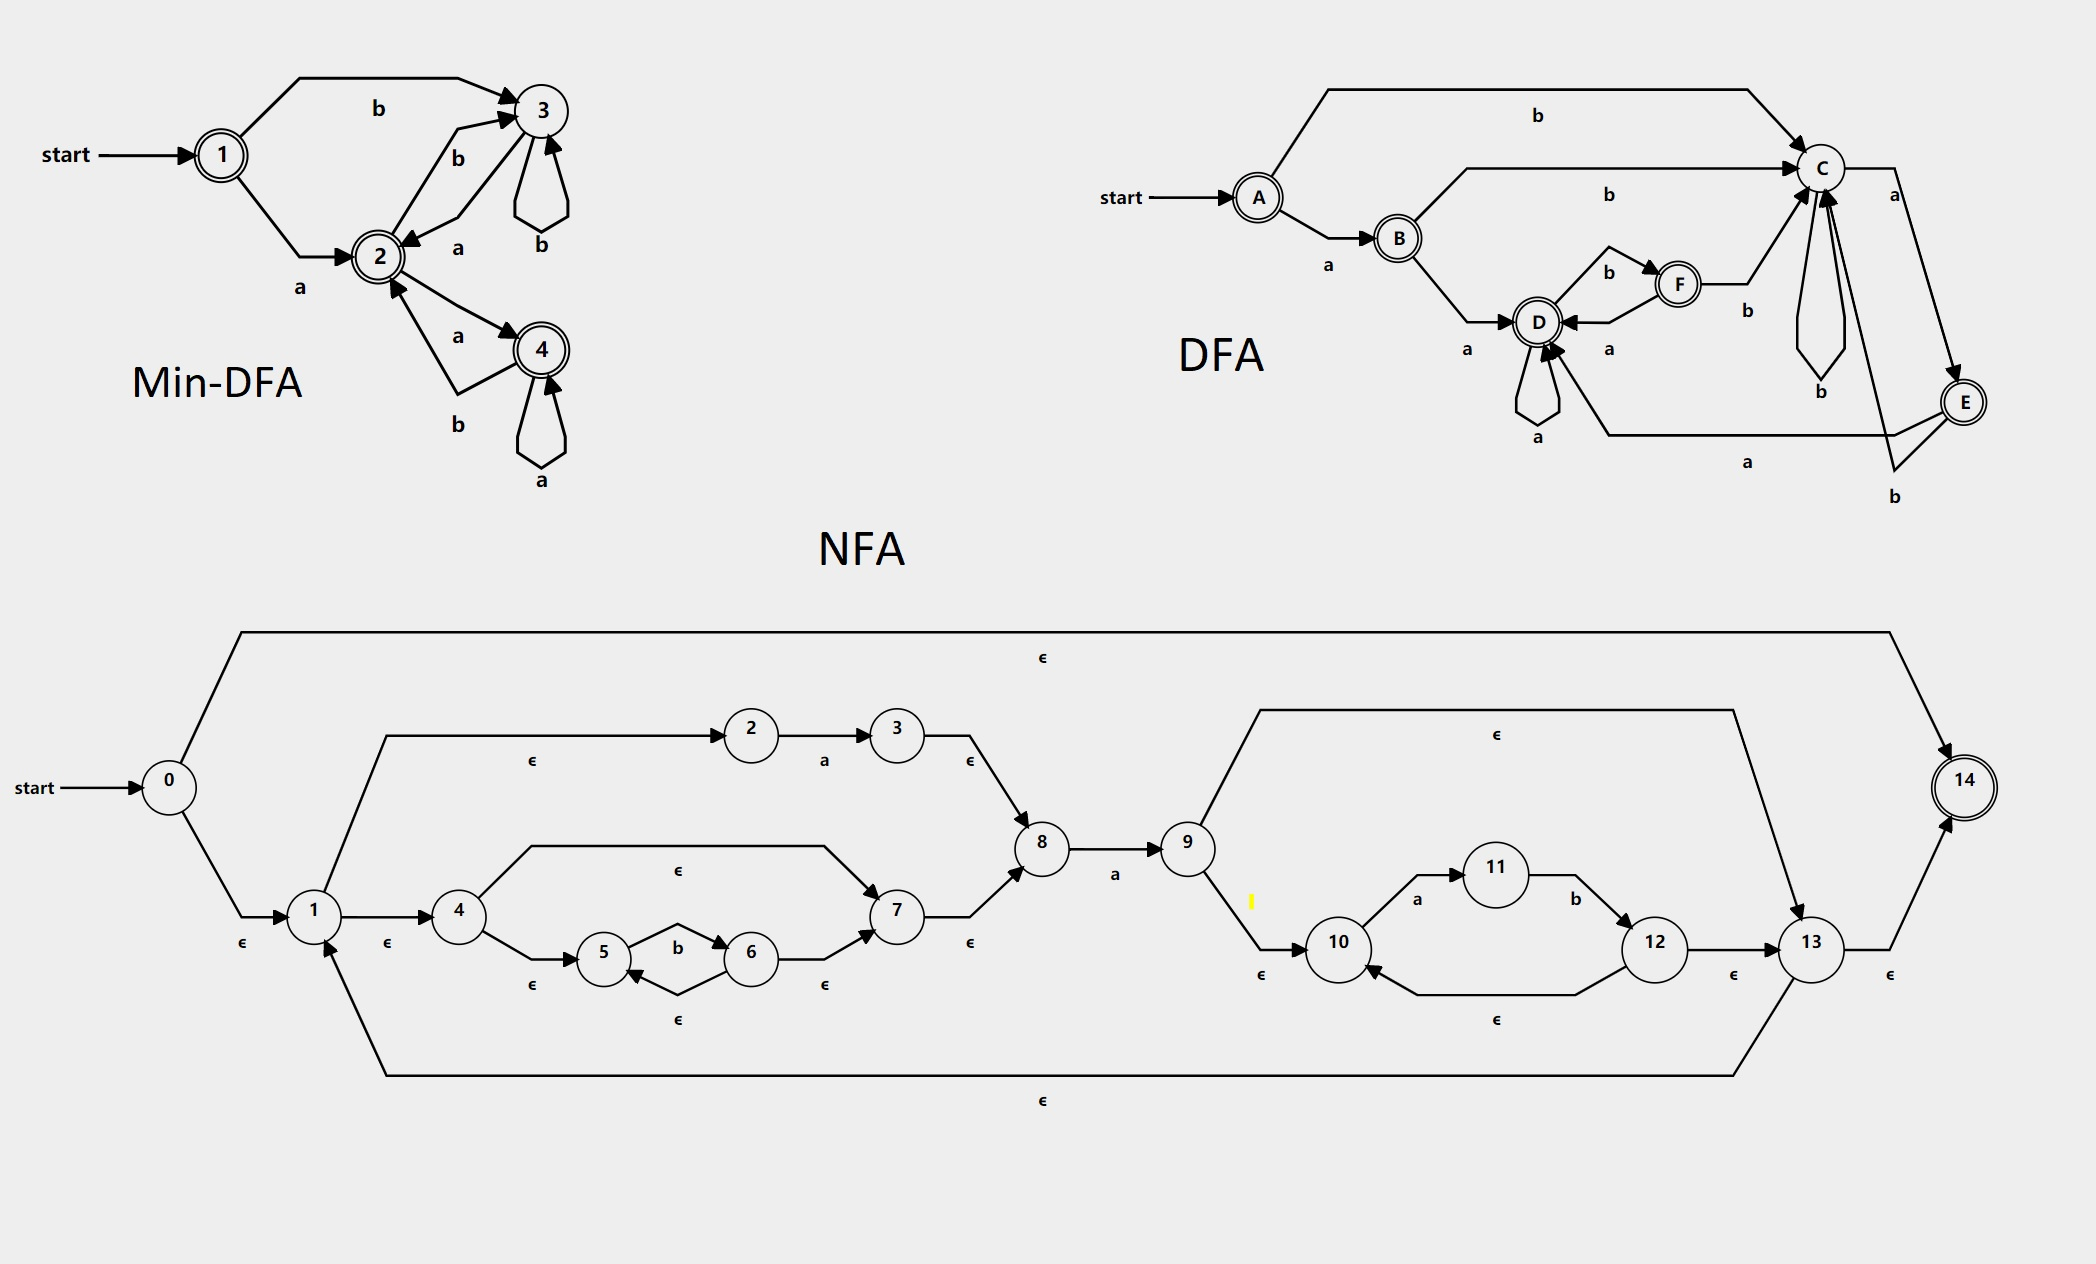
\includegraphics[width=\columnwidth]{mindfa} 
	\caption[]{NFA $ \rightarrow $ DFA $ \rightarrow $ Minimum DFA}
	\label{fig:nfatomindfa} 
\end{figure}

\subsection{NFA to DFA}
In the book "Introduction to the Theory of Computation", a complete algorithm is suggested to convert an epsilon-NFA to a DFA. The conversion, however, is not always minimal; it may be reduced to an even more compact DFA. This section explains the algorithm behind a non-optimum transformation of a desired NFA to corresponding DFA. We get here by calling the function $buildDFA()$ on an arbitrary DFA object, where the algorithm gets the state transition matrix and final and start states of the NFA and passes it to DFA in order to start the conversion procedure.

\subsubsection{Algorithm}
The algorithm is rather straight forward. Starting from an start state, we have to find its epsilon closure, the epsilon closure is a set with respect to a state that includes all the sets to which we may travel from the mentioned state by only moving along the epsilon edges. Then we take a look at the outgoing edges from the epsilon-closure set and complete the state transition matrix of the DFA, by putting the union of outgoing states for a specific symbol in the place of next state in DFA state transition matrix. Finally, we build the set of final states to any state that contains an NFA final state in its state set. To make the case of the algorithm more concrete, we present the main algorithm here.

Suppose there is an NFA N $< Q, \sum, q0, \sigma, F >$ which recognizes a language L. Then the DFA D $< Q', \sum, q0, \sigma, F'>$ can be constructed for language L as:
\begin{enumerate}
	\item Initially $Q' = \emptyset$
	\item Add q0 to Q’.
	\item For each state in Q’, find the possible set of states for each input symbol using transition function of NFA. If this set of states is not in Q’, add it to Q’.
	\item Final state of DFA will be all states with contain F. (final states of NFA)
\end{enumerate}

A simple example of how the algorithm works is given in Figure~\vref{fig:nfatodfaproc}.
\begin{figure}[tb]
	\centering 
	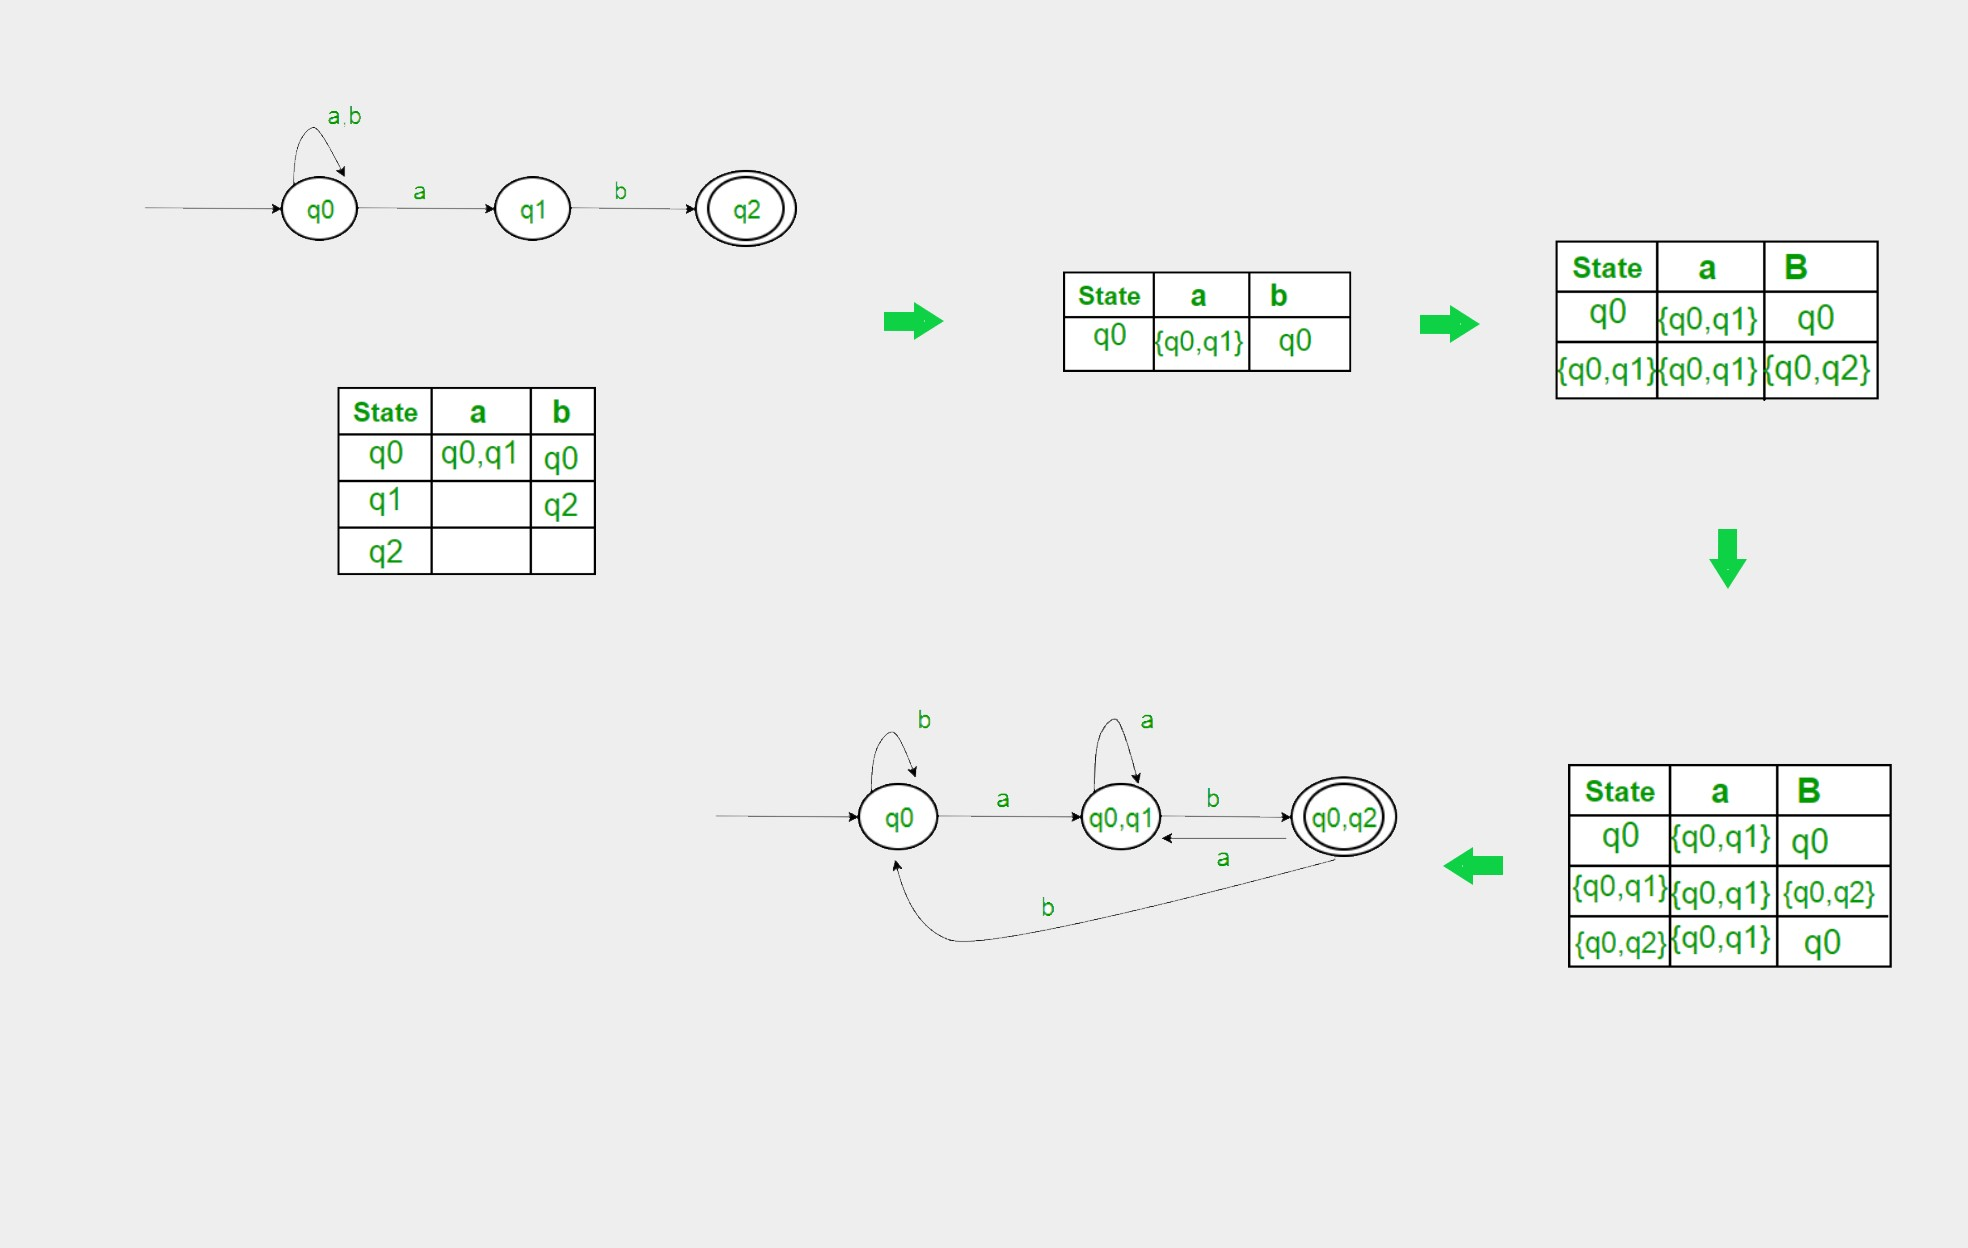
\includegraphics[width=\columnwidth]{nfatodfa} 
	\caption[]{NFA $ \rightarrow $ DFA detailed procedure}
	\label{fig:nfatodfaproc} 
\end{figure}

\subsubsection{Implementation}
The implementation is, as stated before, started with the function $buildDFA$. In this function we first load the state transition matrix of the input NFA, and initialize an empty state transition matrix for our DFA object. 

\paragraph{Adding the alphabet} After the initialization, we add the NFA alphabet to DFA using the function $addNewColumn()$, except for the epsilon sign. The alphabet is added by just simply copying the first column of NFA state transition matrix into the DFA's.

\paragraph{Finding epsilon closures}
Finding the epsilon closures is not an easy task, i.e. it requires to find a set connected to a specific state via epsilon edges, and then also finding the same thing for each of these states. This yields a recursive function, implemented as $getEpsilonClosure()$ to recursively find the epsilon closure set. To avoid getting stuck in a loop we have to keep track of seen states in a separate array.

\paragraph{Filling the state transition matrix}
Next we iterate over the columns of NFA state transition matrix. We keep the index of the last checked column in the variable $lastCheckedColumn$ to help us investigate the columns one by one. During the investigation, whenever we reach a new state we keep its record and later add it as a new column to the DFA state transition matrix. The function $fillColumnFromNFA(lastCheckedColumn)$ performs the union operation on the ongoing states and also updates the epsilon closure for each of the states. The following code gets the most of what is said in this paragraph.

\begin{lstlisting}
/** See where the last state added goes, fill its column,
* add the new states to state transition matrix as well.
*/
int lastCheckedColumn = 0;

/** Continue until there is no new state. */
while (lastCheckedColumn < this.stmax.size() - 1) {

	/** Increase the last checked number. */
	lastCheckedColumn++;
	
	/** Fill the current column. */
	this.fillColumnFromNFA(lastCheckedColumn);
	
	/** Check whether a new state is found and add it. */
	this.addNewStates(lastCheckedColumn);
}
\end{lstlisting}

\paragraph{Simplifying the matrix} After what we performed in the previous code, we now rename the states from the complicated state names like [1,2,3] to simple integers. This state is not necessary but compensates to the reduction of complexity caused by the previous algorithms. We also sort the state numbers for more convenience.

\subsubsection{Results}
In this subsection, we present the results of conversion from NFA to DFA. We are aware that this conversion is only the first step to reach the minimum DFA but the results from this stage will act as a strong ground for the next stage's implementation. The results for a few cases are shown in the next section's result tab, alongside the minimum DFA results.

\subsection{DFA to Minimum DFA}
The term minimization of a DFA refers to converting a given DFA to its equivalent DFA with minimum number of states. To this extent, we use an algorithm to perform the conversion. The algorithm tries to find some partitions which are distinguishable from one another and mark them as correct states. The whole procedure starts with the function $makeMin()$, an attribute of a $DFA$ class. This procedure, same as other operations, is based on manipulation of the state transition matrix to reach a minimized one.
\subsubsection{Algorithm}
The algorithm is mainly based on partitioning. A useful intuition to understand the way it works is to consider the case in which two states become indistinguishable. This happens when they have the same output for every symbol in the alphabet, and by the same output we mean that the output lies in the same partition. If for the first partitioning, we consider final and non-final states and loop over the partitioning procedure using the distinguishable states in each partition, we would finally reach the desired results. Hence, the formal algorithm is as the following.

Suppose there is a DFA D $< Q, \sum, q0, \sigma, F >$ which recognizes a language L. Then the minimized DFA D $< Q', \sum, q0, \sigma', F' >$ can be constructed for language L as:

\begin{enumerate}
\item We will divide Q (set of states) into two sets. One set will contain all final states and other set will contain non-final states. This partition is called $P_0$.
\item Initialize $k = 1$.
\item Find $P_k$ by partitioning the different sets of $P_{k-1}$. In each set of $P_{k-1}$, we will take all possible pair of states. If two states of a set are distinguishable, we will split the sets into different sets in $P_k$.
\item Stop when $P_k$ = $P_{k-1}$. (No change in partition)
\item All states of one set are merged into one. No. of states in minimized DFA will be equal to no. of sets in $P_{k}$.
\end{enumerate}

A simple example of how the algorithm works is given in Figure~\vref{fig:dfatodfamin}.
\begin{figure}[tb]
	\centering 
	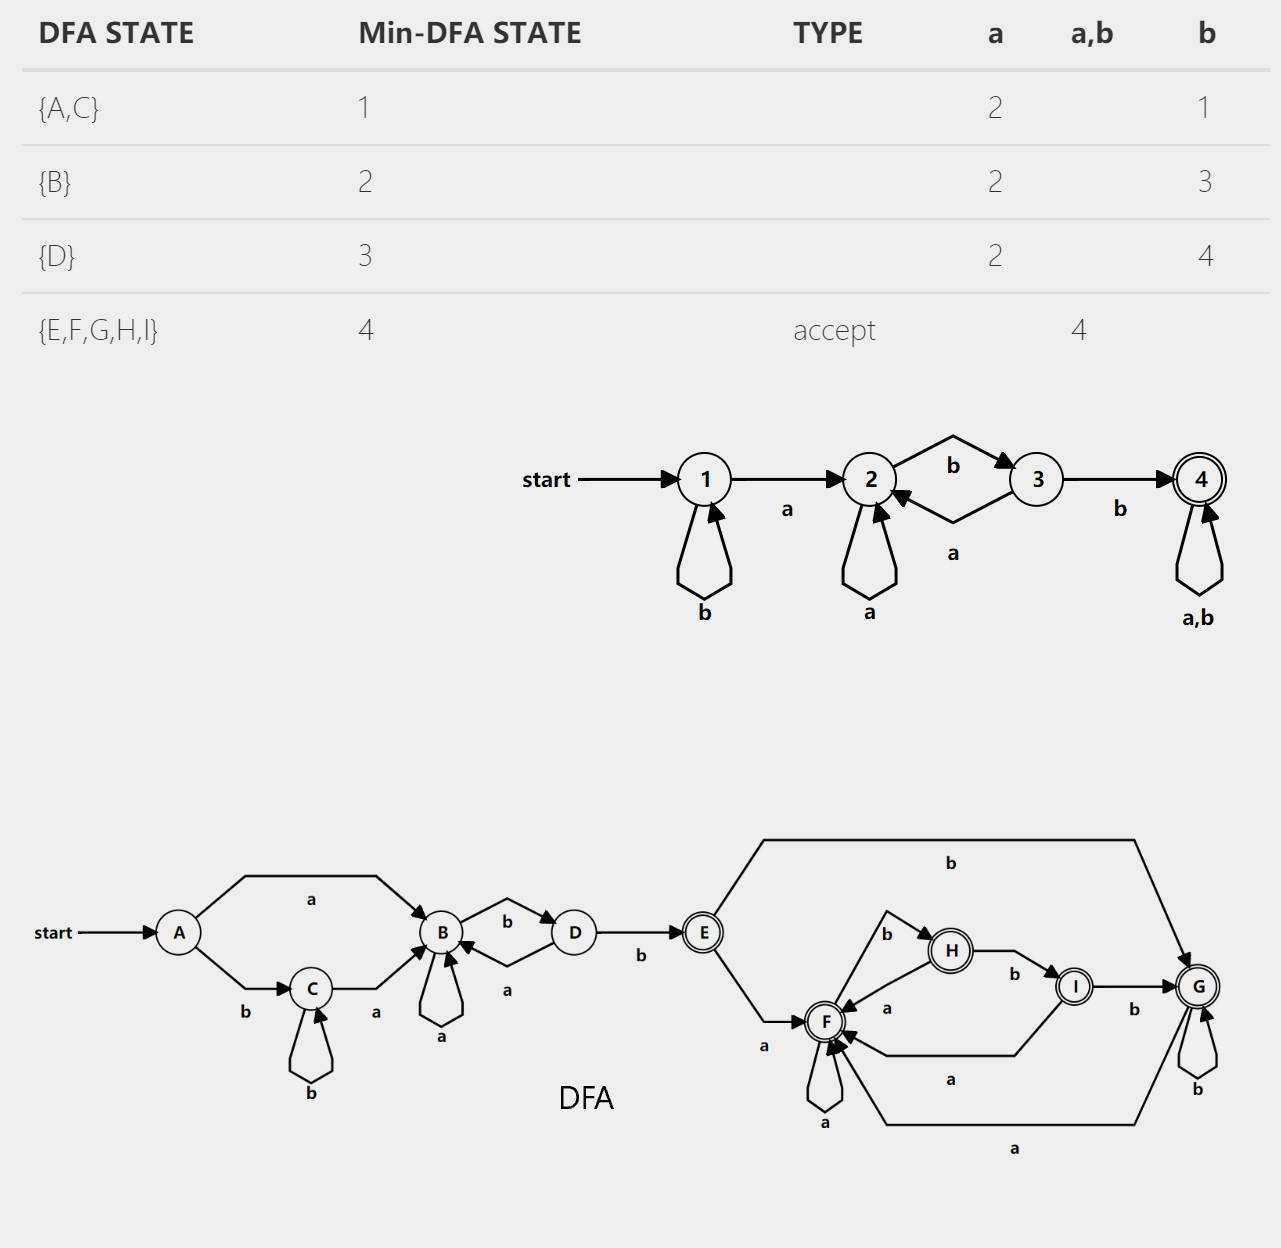
\includegraphics[width=\columnwidth]{dfatomindfaproc} 
	\caption[]{DFA $ \rightarrow $ Minimum DFA detailed procedure}
	\label{fig:dfatodfamin} 
\end{figure}
\subsubsection{Implementation}
The implementation is a bit complicated. To simplify the explanation we start from the base function and explain the big picture of implementation gradually.

\subsubsection{Results}

\section{Context Free Grammar to PDA}
A context free grammar is a grammar which satisfies certain properties. These properties and rules are given true a set of rules called the production rules. A grammar of this kind builds the language also known as formal language. Grammars work by proposing transformations so that we can make to construct a string in the language described by a grammar. Grammars will describe how to convert a start symbol (usually S) into some string of symbols.
\subsubsection{Algorithm}
Every CFG can be converted to an equivalent PDA. The constructed PDA will perform a leftmost derivation of any string accepted by the CFG. Here, and based on the algorithm mentioned in the text book, we convert a CFG to a PDA as mentioned in the following algorithm. However, we remove the two start and end states as here we have an stack initializer and we can also check whether the stack gets empty or not. That said, we now illustrate the algorithm behind the scene.

\begin{enumerate}
	\item Create three states, start, and end.
	\item Fill the stack with the special character \$ and the start variable. namely S.
	\item As for the loop state, for reach rule in the form of $A \rightarrow \omega$ which A is a variable, pop $A$ and push $\omega$. For each terminal, also create the action $a \rightarrow \epsilon$ in the loop state.
	\item Create a transition from loop to the end state when seeing the special character, \$.
\end{enumerate}

An state diagram of the algorithm is shown in the Figure~\vref{fig:cfgtopda}.
\begin{figure}[tb]
	\centering 
	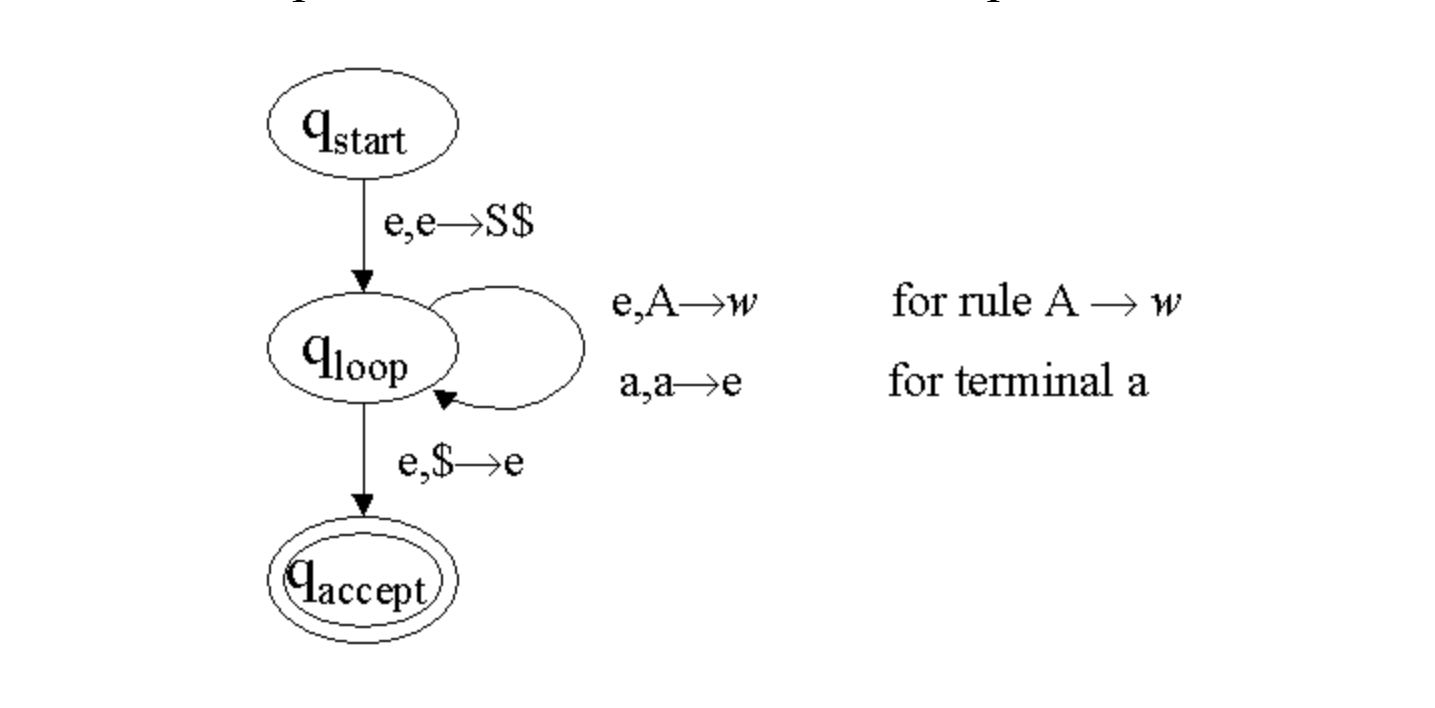
\includegraphics[width=\columnwidth]{cfgtopda} 
	\caption[]{CFG $ \rightarrow $ PDA state diagram}
	\label{fig:cfgtopda} 
\end{figure}


\paragraph{Warning} The initial state of the stack is set to \$. Hence, we do not need to create a transition to put the character inside the stack, based on the discussions previously made about the subject in the class.
\paragraph{Warning} The implementation is not unique. This is crucial to understand in order to evaluate the design and results.
\subsubsection{Implementation}
The implementation of CFG to PDA converter is rather straightforward. Yet, a brief explanation is necessary in order to clarify the various aspects of the design. This function also starts from the main $automata()$ function, detaching from the state machine as a new CFG object. The next paragraphs explain the detailed stages of the design.

The following lines of code would capture most of what is explained in the implementation section.

\begin{lstlisting}
/** See where the last state added goes, fill its column,
* add the new states to state transition matrix as well.
*/
int lastCheckedColumn = 0;

/** Continue until there is no new state. */
while (lastCheckedColumn < this.stmax.size() - 1) {

/** Increase the last checked number. */
lastCheckedColumn++;

/** Fill the current column. */
this.fillColumnFromNFA(lastCheckedColumn);

/** Check whether a new state is found and add it. */
this.addNewStates(lastCheckedColumn);
}
\end{lstlisting}

\paragraph{Parsing the input} Here in the same manner of the previous sections, we again have an object called $CFGEntry$. This object handles the input by saving all the input data in the corresponding fields. Exceptionally, the production rules are saved in a Java HashMap object. The hash map serves to separate the variables from the right hand side of te production rules and converting the right hand side to an $ArrayList<String>$, ready to be used in the next sections.

\paragraph{Building the PDA} Trying to build the PDA, we devide the task into two main functions: $makeDFA()$ and $print()$. In the first function, we create a DFA based on the explained state diagram. For each rule we create the corresponding state transition of DFA and then add it to a list called $DFA$. This is a string ArrayList for easier accessibility. Next, in the print function, we implement the correct procedure to print the output DFA as required by the project document. We also create private fields like epsilon inside the CFG class to keep these strings in touch.
\subsubsection{Results}
\end{document}